\documentclass{beamer}
\mode<presentation>
{
  \usetheme{Madrid}      
  \usecolortheme{seahorse} 
  \usefonttheme{structureitalicserif} 
  \setbeamertemplate{footline}{}
  \setbeamertemplate{caption}[numbered]
} 
\usepackage{tikz}
\setbeamercovered{highly dynamic}

\newcounter{saveenumi}
\newcommand{\seti}{\setcounter{saveenumi}{\value{enumi}}}
\newcommand{\conti}{\setcounter{enumi}{\value{saveenumi}}}
\usetikzlibrary{shapes.geometric,calc,angles,positioning,intersections,quotes,decorations,babel,patterns,fit}
\usepackage{tkz-euclide}
\usetkzobj{all}
\usepackage[english]{babel}
\usepackage[utf8]{inputenc}
\usepackage[T1]{fontenc}
\usepackage{hyperref}
\usepackage{graphics}
\usepackage{hyperref}
\hypersetup{
    colorlinks=true,
    linkcolor=blue,
    filecolor=magenta,      
    urlcolor=cyan,
    pdftitle={Sharelatex Example},
    bookmarks=true,
    pdfpagemode=FullScreen,
}
 
\urlstyle{same}
\graphicspath{ {.//home/lenovo/codes/circle} }
\usepackage{standalone}
\usepackage{gensymb}
\title[Your Short Title]{Excercise}
\author{Pratibha}
\institute{}
\date{3 Jan 2020}

\begin{document}

\begin{frame}
  \titlepage
\end{frame}
\begin{frame}{Miscellaneous Exercises}
\begin{enumerate}
\conti
\item The length of the
minute hand of a clock is 14 cm. Find the area
swept by the minute hand in 5 minutes.\\
\seti
\end{enumerate}
\begin{itemize}
\item \textbf{Solution} :
\item Given r = 14 
\begin{figure}[!ht]
\resizebox{0.5\linewidth}{!}
{
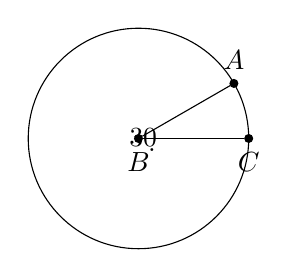
\begin{tikzpicture}
[scale =0.1,>=stealth,point/.style = {draw, circle, fill = black, inner sep = 1pt},]
\node (B) at (0,0)[point,label=below :$B$] {};
\node (C) at (14,0)[point,label=below :$C$] {};
\node (A) at (12.12,6.99)[point,label=above :$A$] {};
\draw (0,0) node [below right] {.} circle (14);
\draw (B)--(A);
\draw (B)--(C);
\tkzMarkAngle[fill=green!40,size=0.1cm,mark=](C,B,A)
\tkzLabelAngle[pos=0.1](C,B,A){\rotatebox{-360}{$30$}}
\end{tikzpicture}


}

\end{figure}


\end{itemize}
\end{frame}
\begin{frame}
\begin{figure}
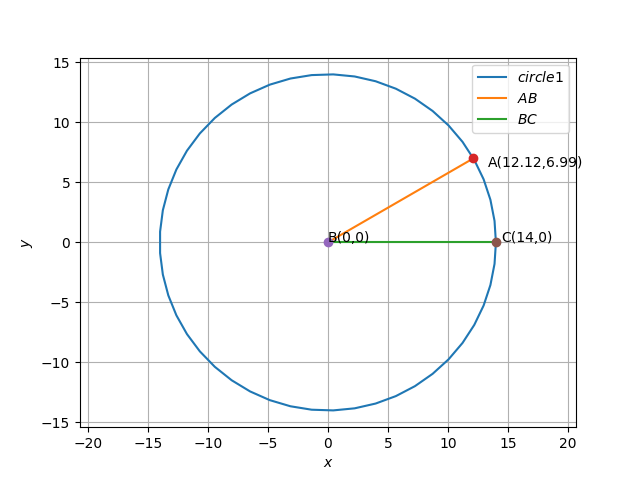
\includegraphics[scale=.6]{./CODES/MISC.png}
\end{figure}
\end{frame}
\begin{frame}

 In 60 minutes minute hand covers  360$\degree$\\
For 5 minutes 6$\degree$ $\times$ 5 = 30$\degree$\\ 
Here $\theta$ = 30 $\degree$ and r = 14cm\\

\begin{align*}
	\text{Area of sector} = \frac{\theta}{360} \times \pi r^2
	=51.31cm^2.
\end{align*}   
\begin{itemize}
\item \url {https://github.com/pratibha444/GEOMETRY/blob/master/CODES/MISC.py} 
\end{itemize}             
\end{frame}
\begin{frame}{Quadrilateral excercise}
\begin{enumerate}
\conti
\item A farmer was having a field in the form of a
parallelogram PQRS . She took any point A on
RS and joined it to points P and Q. In how
many parts the fields is divided? What are the
shapes of these parts? The farmer wants to sow
wheat and pulses in equal portions of the field
separately. How should she do it?
\seti
\end{enumerate}
\begin{itemize}
\item \textbf{Solution} :
\end{itemize}
\begin{center}
\documentclass{article}
\usepackage{tikz}
\usetikzlibrary{shapes.geometric,calc,angles,positioning,intersections,quotes,decorations,babel,patterns,fit}
\usepackage{tkz-euclide}
\usetkzobj{all}
\begin{document}
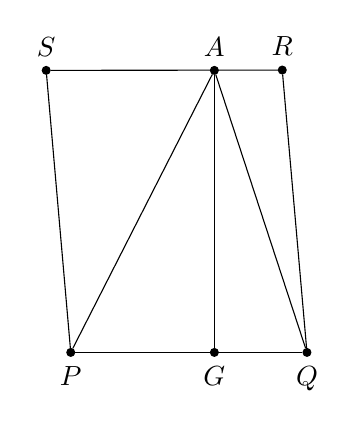
\begin{tikzpicture}
[scale =0.6,>=stealth,point/.style = {draw, circle, fill = black, inner sep = 1pt},]
\node (S) at (-0.52,5.97)[point,label=above :$S$] {};
\node (P) at (0,0)[point,label=below :$P$] {};
\node (A) at (3.04,5.97)[point,label=above :$A$] {};
\node (R) at (4.477,5.977)[point,label=above :$R$] {};
\node (G) at (3.04,0)[point,label=below:$G$] {};
\node (Q) at (5,0)[point,label=below :$Q$] {};
\draw (S)--(P);
\draw (P)--(Q);
\draw (Q)--(R);
\draw (R)--(S);
\draw (A)--(P);
\draw (A)--(Q);
\draw (A)--(G);
\end{tikzpicture}
\end{document}
\end{center}
\end{frame}
\begin{frame}
\begin{itemize}
\item  After joining the point A to p and Q, the feild is divided into 3 parts.\\
\item All the three parts are in triangle shape.\\
As PQRS is a parallelogram so\\
\end{itemize}
\begin{align*}
\textit{Area of PQRS} = \textit{Area of} \triangle{APS} + \triangle{ARQ} + \triangle{PAQ} --(1)\\
\textit{Area of triangle is half of parallelogram}\\\textit{if they have same base and lie between same parallel lines}. \\
\textit{Area of} \triangle{PAQ} = \frac{1}{2} \textit{Area of PQRS}\\
\triangle{PAQ} = \frac{1}{2}\textit{area}(\triangle{APS} + \triangle{ARQ} + \triangle{APQ}\\
2\triangle{PAQ} - \triangle{PAQ} = \textit{area(}\triangle{APS} + \triangle{ARQ}\textit{)}\\
\triangle{PAQ} = \triangle{APS} + \triangle{ARQ}\\
\textit{Hence the farmer can sow wheat in} \triangle{PAQ} \textit{and pulses in} \triangle{APS} and \triangle{ARQ}\\
\end{align*}
\end{frame}
\begin{frame}
\begin{figure}
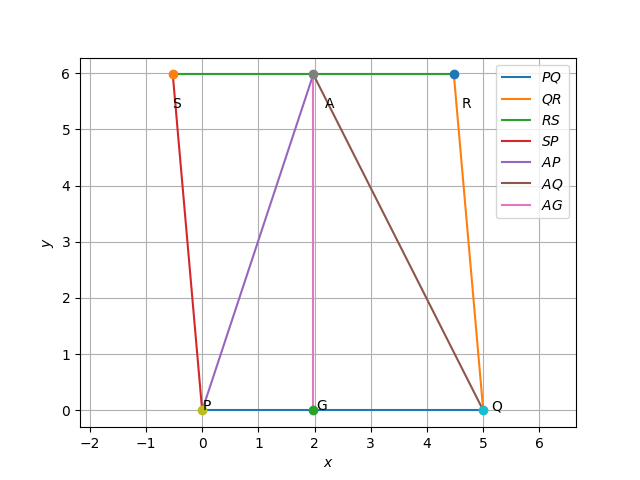
\includegraphics[scale=.5]{./CODES/quad/QUADCON.png}\\
\begin{itemize}
\item \url{https://github.com/pratibha444/GEOMETRY/blob/master/figs/FARM.tex}\\
\item \url{https://github.com/pratibha444/GEOMETRY/blob/master/CODES/quad/QUAD_EXCERCISE.py}
\end{itemize}
\end{figure}
\end{frame}

\begin{frame}{Circle construction}

 Construct a tangent to a circle of radius 4 units
from a point on the concentric circle of radius
6 units.\\
\begin{itemize}
\item\textbf{Solution} :\\
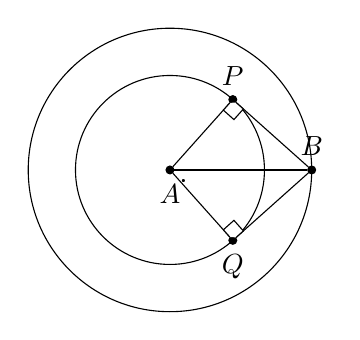
\begin{tikzpicture}
[scale =0.3,>=stealth,point/.style = {draw, circle, fill = black, inner sep = 1pt},]
\node (A) at (0,0)[point,label=below :$A$] {};
\node (P) at (2.66,2.98)[point,label=above :$P$] {};
\node (B) at (6,0)[point,label=above :$B$] {};
\node (Q) at (2.66,-2.98)[point,label=below :$Q$] {};
\draw (0,0) node [below right] {.} circle (6);
\draw (0,0) node [below right] {.} circle (4);
\draw (B)--(A);
\draw (B)--(Q);
\draw (B)--(P);
\draw (A)--(P);
\draw (A)--(Q);
\tkzMarkRightAngle[fill=white!45,size=.6,mark=](B,P,A)
\tkzMarkRightAngle[fill=white!45,size=.6,mark=](B,Q,A)
\end{tikzpicture}
\\  PB and QB are the tangents 
\end{itemize}
\seti
\end{frame}

\begin{frame}
\begin{itemize}
\item \textbf{Given} : r1=4 and r2 = 6\\
\begin{align*}
a=\sqrt{r2^2 - r1^2}\\
a=4.47\\
c=r1 , b=r2\\
p=\frac{b^2+c^2-a^2}{2b}\\
p=2.66\\
q=\sqrt{c^2 - p^2}\\
q=2.98\\
AB = r2 \\
P = (2.66,2.98)\\
Q = (2.66,-2.98)
\end{align*}
\end{itemize}

\end{frame}


\begin{frame}
\begin{figure}
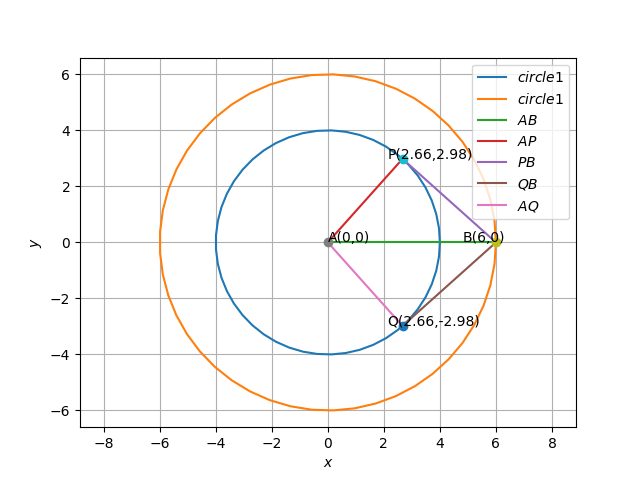
\includegraphics[scale=.4]{./CODES/circle/CIR_CON.png}
\end{figure}
\begin{itemize}
\item \url{https://github.com/pratibha444/GEOMETRY/blob/master/figs/CIRCLE_CON.tex}  \\
\item \url{https://github.com/pratibha444/GEOMETRY/blob/master/CODES/circle/circon.py}
\end{itemize}
\end{frame}
\begin{frame}{Triangle construction}
\begin{enumerate}
\conti
\item Construct an isosceles triangle in which the lengths of the equal sides is 6.5 and the angle between them is 110$\degree$
\seti
\end{enumerate}
\begin{itemize}
\item\textbf{Solution}\\
\begin{tikzpicture}
[scale =0.6,>=stealth,point/.style = {draw, circle, fill = black, inner sep = 1pt},]
\node (B) at (0,0)[point,label=below :$B$] {};
\node (A) at (-2.223,6.108)[point,label=above :$A$] {};
\node (C) at (6.5,0)[point,label=below :$C$] {};
\draw (A)--(B);
\draw (B)--(C);
\draw (C)--(A);
\tkzMarkAngle[fill=green!40,size=0.5cm,mark=](C,B,A)
\tkzLabelAngle[pos=1](C,B,A){\rotatebox{-360}{$110$}}
\end{tikzpicture}

\item BC = 6.5 \item AC = 10.64
\item AB = 6.5\\
\item $\angle B$ = 110\\ 
\end{itemize}
\end{frame}
\begin{frame}
\begin{itemize}
\item\textbf{Given}: BC = 6.5 and AB = 6.5\\
$\angle$ABC = 110
\begin{align*}
a = 6.5 and  c = 6.5\\
b = \sqrt{a^2 + c^2 - 2ac cos(A)}\\
b= 10.64\\
p=\frac{a^2 + c^2 - b^2}{2a}\\
p=-2.22\\
q=\sqrt{c^2 - p^ 2}\\
q = 6.10
\end{align*}
\end{itemize}
\end{frame}

\begin{frame}
\begin{figure}
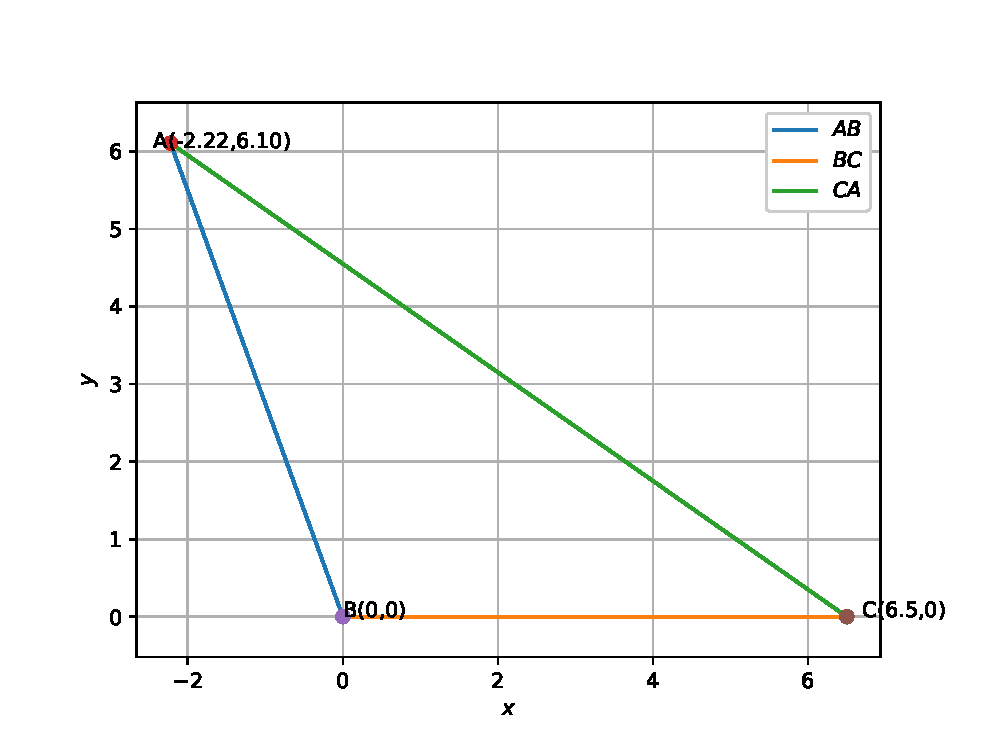
\includegraphics[scale=.4]{./figs/TRI_CON.eps}
\end{figure}
\begin{itemize}
\item \url{https://github.com/pratibha444/GEOMETRY/blob/master/figs/tri_iso.tex}
\item \url{https://github.com/pratibha444/GEOMETRY/blob/master/CODES/triangle/TRI_CON.py}
\end{itemize}
\end{frame}

\end{document}